The output of the data processing described in \sref{data} is the data set $X$,
which is split into three parts: $X_1$ is for training, $X_2$ for validation,
and $X_3$ for testing. In what follows, we elaborate on the processes that are
taking place during these three stages of working with the model in
\sref{model}.

\subsection{Training}
The model outlined in \sref{model} has a large number of parameters that have to
be learned; for this purpose, $X_1$ is utilized. The training is undertaken
using the so-called backpropagation through time using stochastic gradient
descent \cite{goodfellow2016}. The variant of gradient descent that we use is
Adam \cite{kingma2014}, which is an adaptive optimization method. There are two
important aspects about training to be discussed.

\begin{figure}[t]
  \centering
  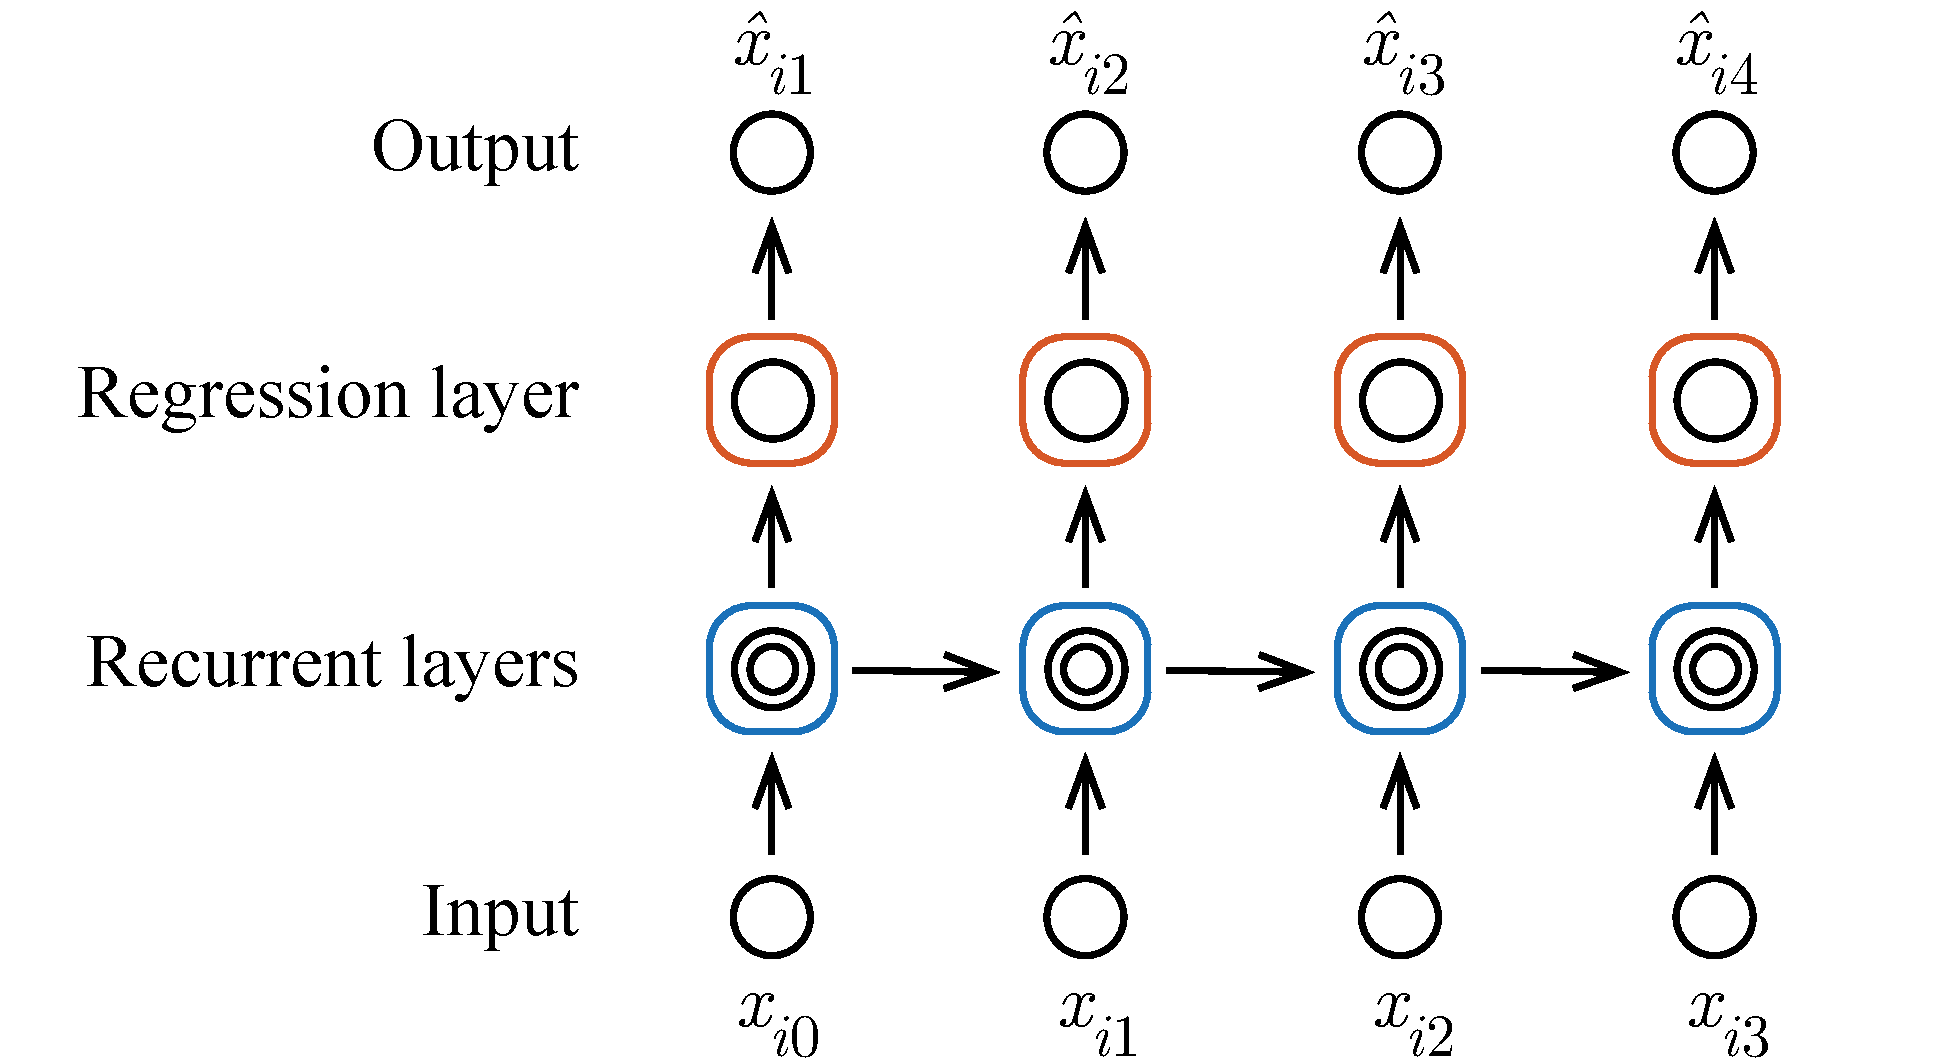
\includegraphics[width=1.0\columnwidth]{include/assets/figures/unroll.pdf}
  \vspace{-2.0em}
  \caption{Example of dynamic unrolling during the model's usage.}
  \vspace{-1.5em}
  \flab{unroll}
\end{figure}

The first concerns the way a single resource-usage trace is fed into the model.
First, note that a trace has multiple data points ($l_i > 1$), and that two
traces are of different lengths in general ($l_i \neq l_j$) since the execution
times of different tasks can differ substantially. All the points of a trace are
fed in one pass using a technique called dynamic unrolling. An illustration for
$l_i = 4$ is given in \fref{unroll}, in which the representation in \fref{model}
has been simplified even further and put on a side. It can be seen that the
model has been replicated as many times are there are data points in the trace.
However, it is still the same model, and all the replicas share the same
parameters. It can also be seen in \fref{unroll} how information flows from one
step to the next, which is what makes the model recurrent.

Now, it is not efficient to feed only one trace at a time due to the inevitable
overhead imposed by the computations involved. Therefore, calculations should be
performed in batches whenever possible. Since $l_i \neq l_j$ in general, it is
not possible to stack multiple arbitrary traces into a single tensor directly.
In order to circumvent this, we reside to bucketing. Specifically, each read
trace is put into one of many queues based on its length. When a queue
accumulates the desired number of traces---referred to as the batch size---it
emits a batch to be further consumed by the model.

\subsection{Validation}
To this end, we use the Hyperband algorithm \cite{li2016}.

\subsection{Testing}
In order to have a long-range prediction (multiple steps ahead), we use
refeeding: the predicted value $\hat{x}_{i,k + 1}$ is fed into the model as if
it was the actual resource usage $x_{i,k + 1}$ at step $k + 1$, which is not
yet known at time step $k$. The process continues until all the desired $h$
future values are estimated.
